This chapter presents a simulation study results and the analysis of a
real-based dataset.

\section{SIMULATION STUDY}
\label{cap:simures}

\begin{figure}[H]
 \setlength{\abovecaptionskip}{.0001pt}
 \caption{BUILDING \(\Sigma\)}
 \vspace{0.5cm}\centering
\begin{aligned}
 \Sigma_{~4\times 4} = \begin{bmatrix} R & C\\
                                     C & T
                     \end{bmatrix} \quad \text{with} \quad
 R_{~2\times 2},~T_{~2\times 2},~\text{and}~C_{~2\times 2}, \quad
 \text{all symmetric matrices}.\\
 R~\text{from \textbf{risk level}, that can be}\\
 \text{The same for}~T,~\text{from \textbf{trajectory time}}.
\end{aligned}\\
 \vspace{0.5cm}
 \begin{footnotesize}
  SOURCE: The author (2021).
 \end{footnotesize}
 \label{fig:buildingSigma}
\end{figure}

\autoref{tab:models1} and \autoref{tab:models2}

\newcolumntype{g}{>{\columncolor{Gray}}c}
\begin{table}[H]
 \centering
 \setlength{\abovecaptionskip}{.0001pt}
 \caption{MODELS, FIRST PART}
 \label{tab:models1}
 \vspace{0.2cm}
 \begin{small}
 \begin{tabular}{r|cccccccc|r}
  \toprule
  \multirow{3}{*}{\textbf{Label}} &
  \multicolumn{2}{c}{\textbf{\makecell{Risk\\level}}} &
  \multicolumn{2}{c}{\textbf{\makecell{Trajectory\\time}}} &
  \multirow{3}{*}{\textbf{\makecell{Risk\\corr}}} &
  \multirow{3}{*}{\textbf{\makecell{Time\\corr}}} &
  \multirow{3}{*}{\textbf{\makecell{1st order\\risk/time\\interaction}}} &
  \multirow{3}{*}{\textbf{\makecell{2nd order\\risk/time\\interaction}}} &
  \multirow{3}{*}{\textbf{\makecell{Number of\\parameters}}}\\
  \cmidrule{2-3} \cmidrule{4-5}
  & \(\bm{=}\) & \(\bm{\neq}\)
  & \(\bm{=}\) & \(\bm{\neq}\) & & & & &\\
  \midrule
  model1 & \Checkmark & & & & & & & & 7\\
  \midrule
  model2 & & \Checkmark & & & & & & & 8\\
  \midrule
  model3 & \Checkmark & & & & \Checkmark & & & & 8\\
  \midrule
  model4 & & \Checkmark & & & \Checkmark & & & & 9\\
  \midrule
  model5 & & & \Checkmark & & & & & & 7\\
  \midrule
  model6 & & & & \Checkmark & & & & & 8\\
  \midrule
  model7 & & & \Checkmark & & & \Checkmark & & & 8\\
  \midrule
  model8 & & & & \Checkmark & & \Checkmark & & & 9\\
  \midrule
  model9 & \Checkmark & & \Checkmark & & & & & & 8\\
  \midrule
  model10 & & \Checkmark & & \Checkmark & & & & & 10\\
  \midrule
  model11 & \Checkmark & & \Checkmark & & \Checkmark & & & & 9\\
  \midrule
  model12 & & \Checkmark & & \Checkmark & \Checkmark & & & & 11\\
  \midrule
  model13 & \Checkmark & & \Checkmark & & & \Checkmark & & & 9\\
  \midrule
  model14 & & \Checkmark & & \Checkmark & & \Checkmark & & & 11\\
  \midrule
  model15 &
  \Checkmark & & \Checkmark & & \Checkmark & \Checkmark & & & 10\\
  \midrule
  model16 &
  & \Checkmark & & \Checkmark & \Checkmark & \Checkmark & & & 12\\
  \midrule
  model17 &
  \Checkmark & & \Checkmark & & \Checkmark & \Checkmark &
  \Checkmark & & 11\\
  \midrule
  model18 &
  & \Checkmark & & \Checkmark & \Checkmark & \Checkmark &
  \Checkmark & & 13\\
  \midrule
  model19 &
  \Checkmark & & \Checkmark & & \Checkmark & \Checkmark &
  \Checkmark & & 11\\
  \midrule
  model20 &
  & \Checkmark & & \Checkmark & \Checkmark & \Checkmark &
  \Checkmark & & 13\\
  \bottomrule
 \end{tabular}
 \end{small}
\begin{footnotesize}
 \begin{flushleft}
  SOURCE: The author (2021).
 \end{flushleft}
\end{footnotesize}
\end{table}

\newcolumntype{g}{>{\columncolor{Gray}}c}
\begin{table}[H]
 \centering
 \setlength{\abovecaptionskip}{.0001pt}
 \caption{MODELS, SECOND AND LAST PART}
 \label{tab:models2}
 \vspace{0.2cm}
 \begin{small}
 \begin{tabular}{r|cccccccc|r}
  \toprule
  \multirow{3}{*}{\textbf{Label}} &
  \multicolumn{2}{c}{\textbf{\makecell{Risk\\level}}} &
  \multicolumn{2}{c}{\textbf{\makecell{Trajectory\\time}}} &
  \multirow{3}{*}{\textbf{\makecell{Risk\\corr}}} &
  \multirow{3}{*}{\textbf{\makecell{Time\\corr}}} &
  \multirow{3}{*}{\textbf{\makecell{1st order\\risk/time\\interaction}}} &
  \multirow{3}{*}{\textbf{\makecell{2nd order\\risk/time\\interaction}}} &
  \multirow{3}{*}{\textbf{\makecell{Number of\\parameters}}}\\
  \cmidrule{2-3} \cmidrule{4-5}
  & \(\bm{=}\) & \(\bm{\neq}\)
  & \(\bm{=}\) & \(\bm{\neq}\) & & & & &\\
  \midrule
  model21 &
  \Checkmark & & \Checkmark & & \Checkmark & \Checkmark &
  \Checkmark \Checkmark & & 12\\
  \midrule
  \rowcolor[gray]{.9}
  \textbf{model22} &
  & \Checkmark & & \Checkmark & \Checkmark & \Checkmark &
  \Checkmark \Checkmark & & 14\\
  \midrule
  model23 &
  \Checkmark & & \Checkmark & & & & \Checkmark & & 9\\
  \midrule
  model24 &
  & \Checkmark & & \Checkmark & & & \Checkmark & & 11\\
  \midrule
  model25 &
  \Checkmark & & \Checkmark & & \Checkmark & & \Checkmark & & 10\\
  \midrule
  model26 &
  & \Checkmark & & \Checkmark & \Checkmark & & \Checkmark & & 12\\
  \midrule
  model27 &
  \Checkmark & & \Checkmark & & & \Checkmark & \Checkmark & & 10\\
  \midrule
  model28 &
  & \Checkmark & & \Checkmark & & \Checkmark & \Checkmark & & 12\\
  \midrule
  model29 &
  \Checkmark & & \Checkmark & & & & \Checkmark \Checkmark & & 10\\
  \midrule
  model30 &
  & \Checkmark & & \Checkmark & & & \Checkmark \Checkmark & & 12\\
  \midrule
  model31 &
  \Checkmark & & \Checkmark & & \Checkmark & &
  \Checkmark \Checkmark & & 11\\
  \midrule
  model32 &
  & \Checkmark & & \Checkmark & \Checkmark & &
  \Checkmark \Checkmark & & 13\\
  \midrule
  model33 &
  \Checkmark & & \Checkmark & & & \Checkmark &
  \Checkmark \Checkmark & & 11\\
  \midrule
  model34 &
  & \Checkmark & & \Checkmark & & \Checkmark &
  \Checkmark \Checkmark & & 13\\
  \midrule
  model35 &
  \Checkmark & & \Checkmark & & \Checkmark & \Checkmark &
  \Checkmark \Checkmark & \Checkmark \Checkmark & 14\\
  \midrule
  \rowcolor[gray]{.9}
  \textbf{model36} &
  & \Checkmark & & \Checkmark & \Checkmark & \Checkmark &
  \Checkmark \Checkmark & \Checkmark \Checkmark & 16\\
  \midrule
  model37 &
  \Checkmark & & \Checkmark & & \Checkmark & \Checkmark & &
  \Checkmark \Checkmark & 12\\
  \midrule
  \rowcolor[gray]{.9}
  \textbf{model38} &
  & \Checkmark & & \Checkmark & \Checkmark & \Checkmark & &
  \Checkmark \Checkmark & 14\\
  \midrule
  model39 &
  \Checkmark & & \Checkmark & & & &
  \Checkmark \Checkmark & \Checkmark \Checkmark & 12\\
  \midrule
  \rowcolor[gray]{.9}
  \textbf{model40} &
  & \Checkmark & & \Checkmark & & &
  \Checkmark \Checkmark & \Checkmark \Checkmark & 14\\
  \bottomrule
 \end{tabular}
 \end{small}
\begin{footnotesize}
 \begin{flushleft}
  SOURCE: The author (2021).
 \end{flushleft}
\end{footnotesize}
\end{table}

\begin{figure}[H]
 \setlength{\abovecaptionskip}{.0001pt}
 \caption{PARAMETERS BIAS WITH 2.5\% AND 97.5\% QUANTILES}
 \vspace{0.2cm}\centering
 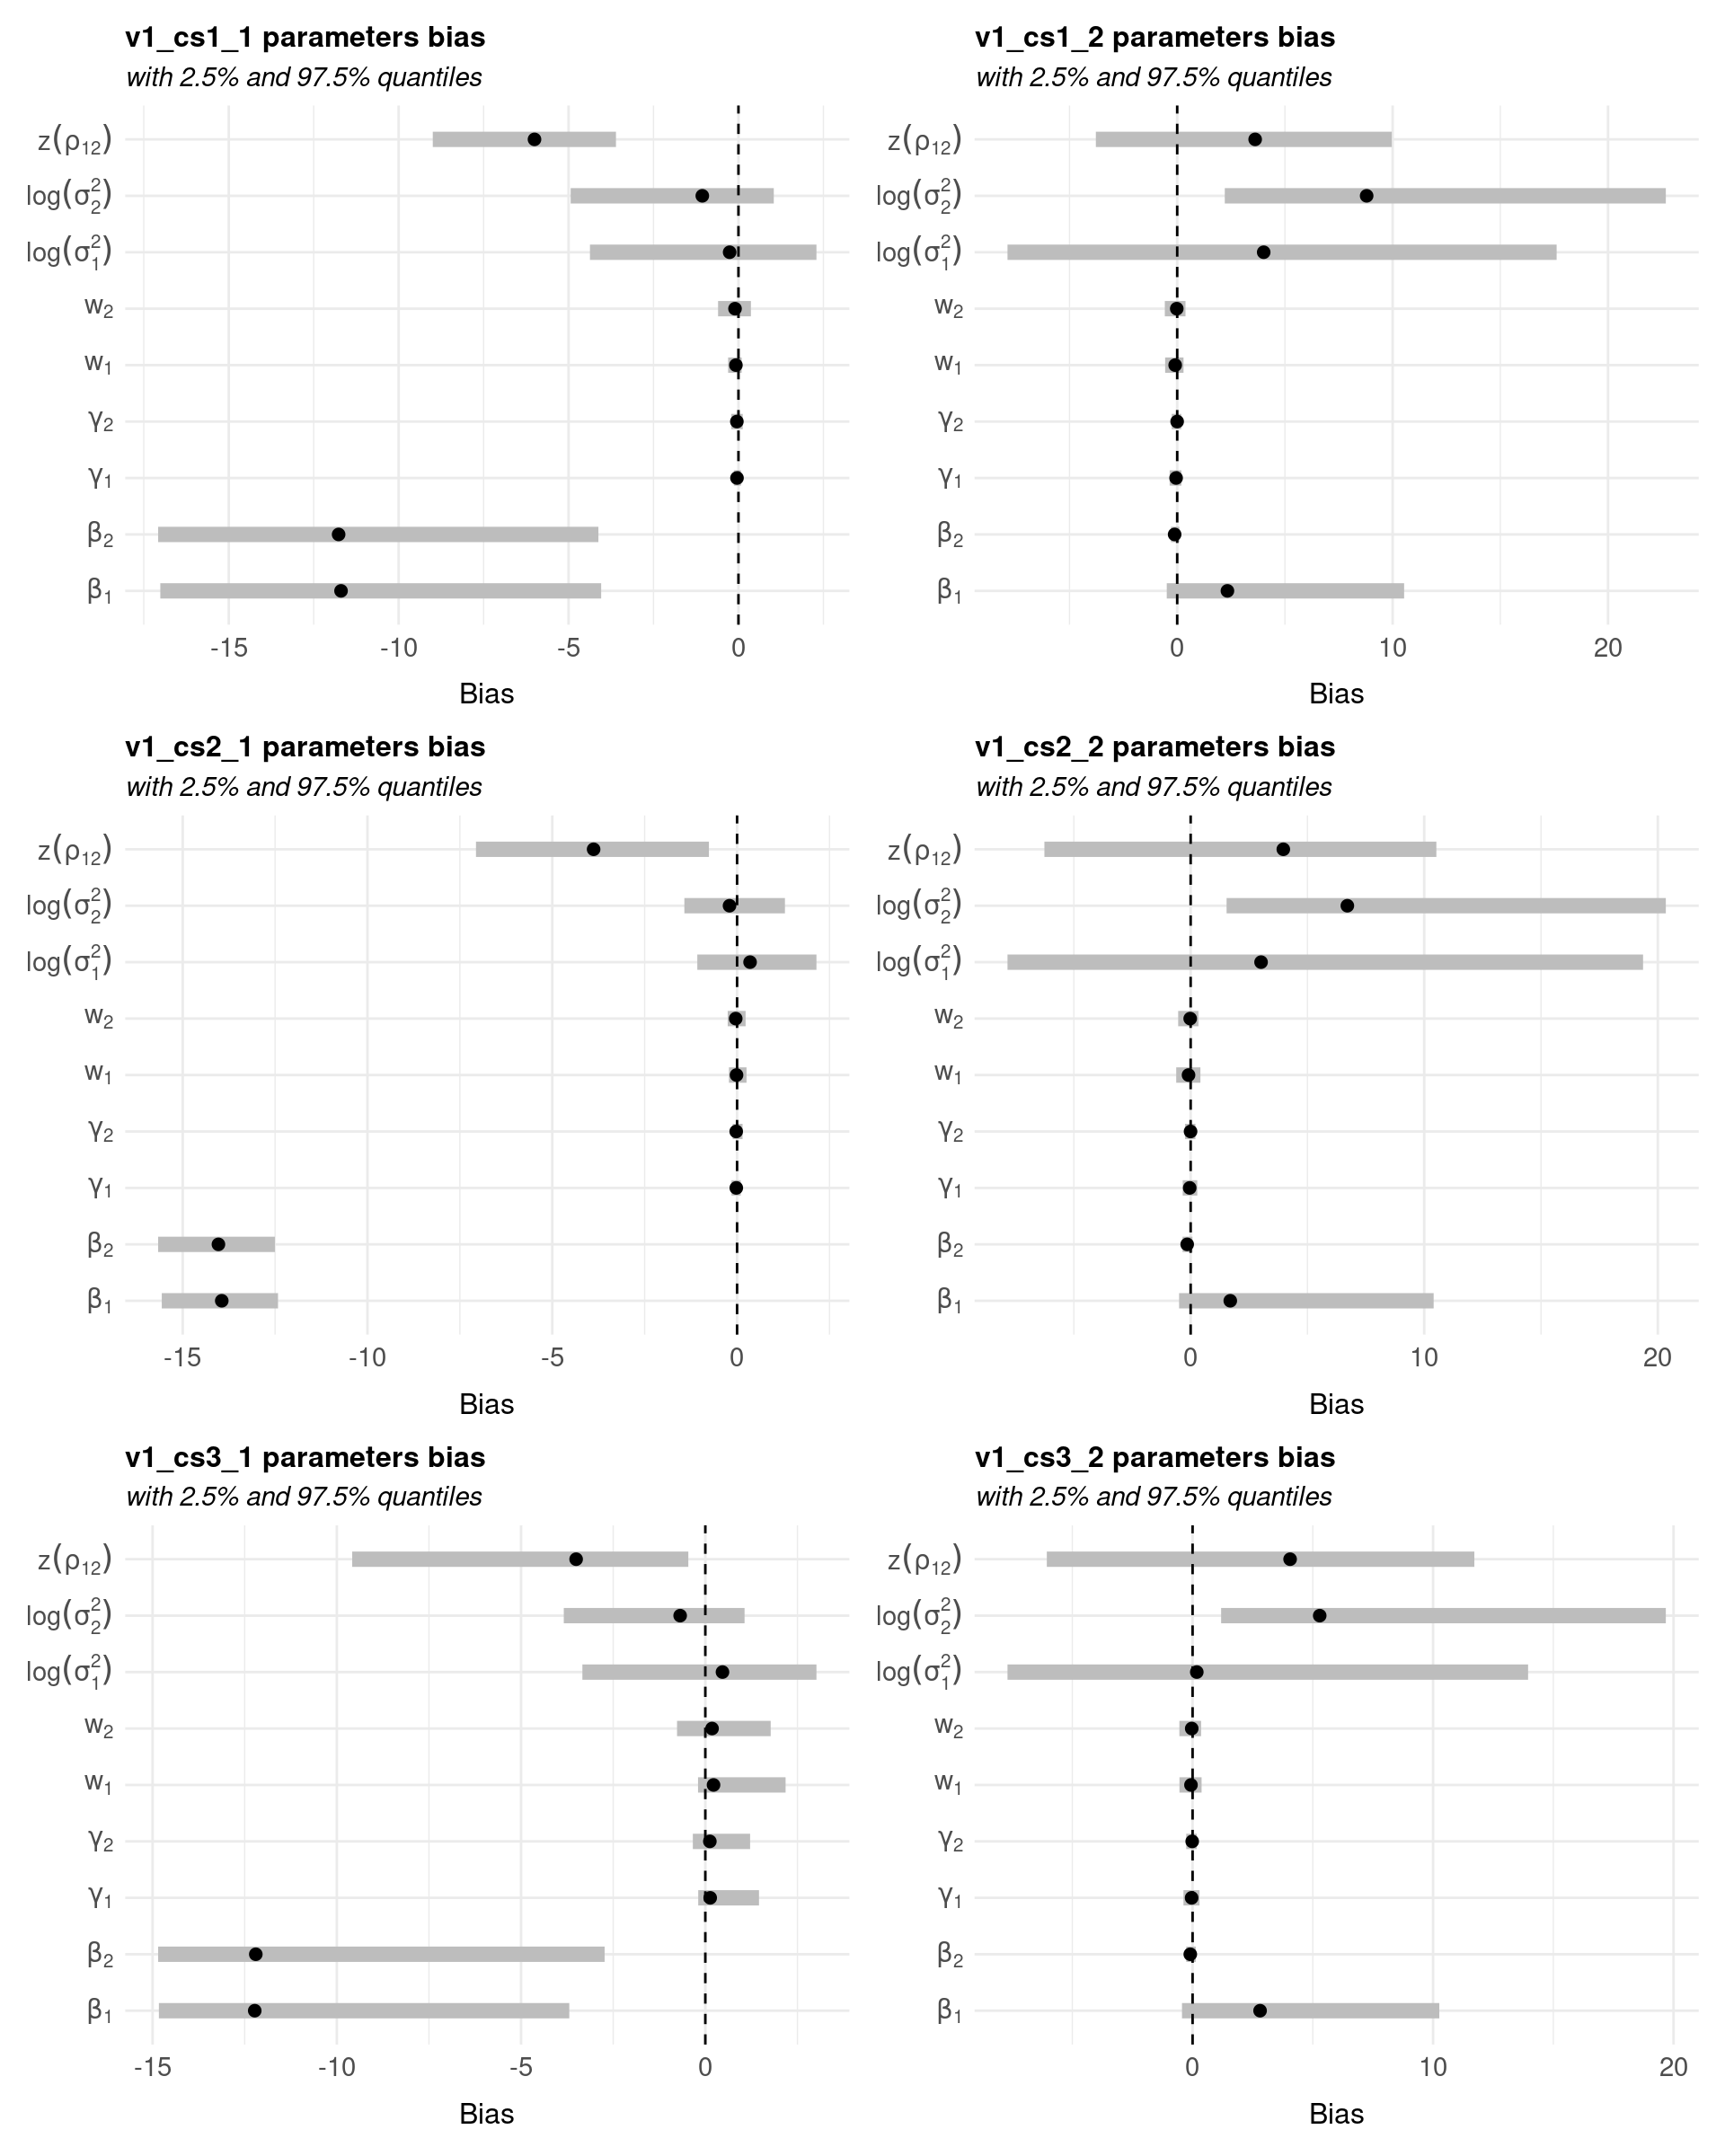
\includegraphics[width=\textwidth]{bias2plot-1.png}\\
 \begin{footnotesize}
  SOURCE: The author (2021).
 \end{footnotesize}
 \label{fig:bias2plot}
\end{figure}

\begin{figure}[H]
 \setlength{\abovecaptionskip}{.0001pt}
 \caption{PARAMETERS CORRELATION}
 \vspace{0.2cm}\centering
 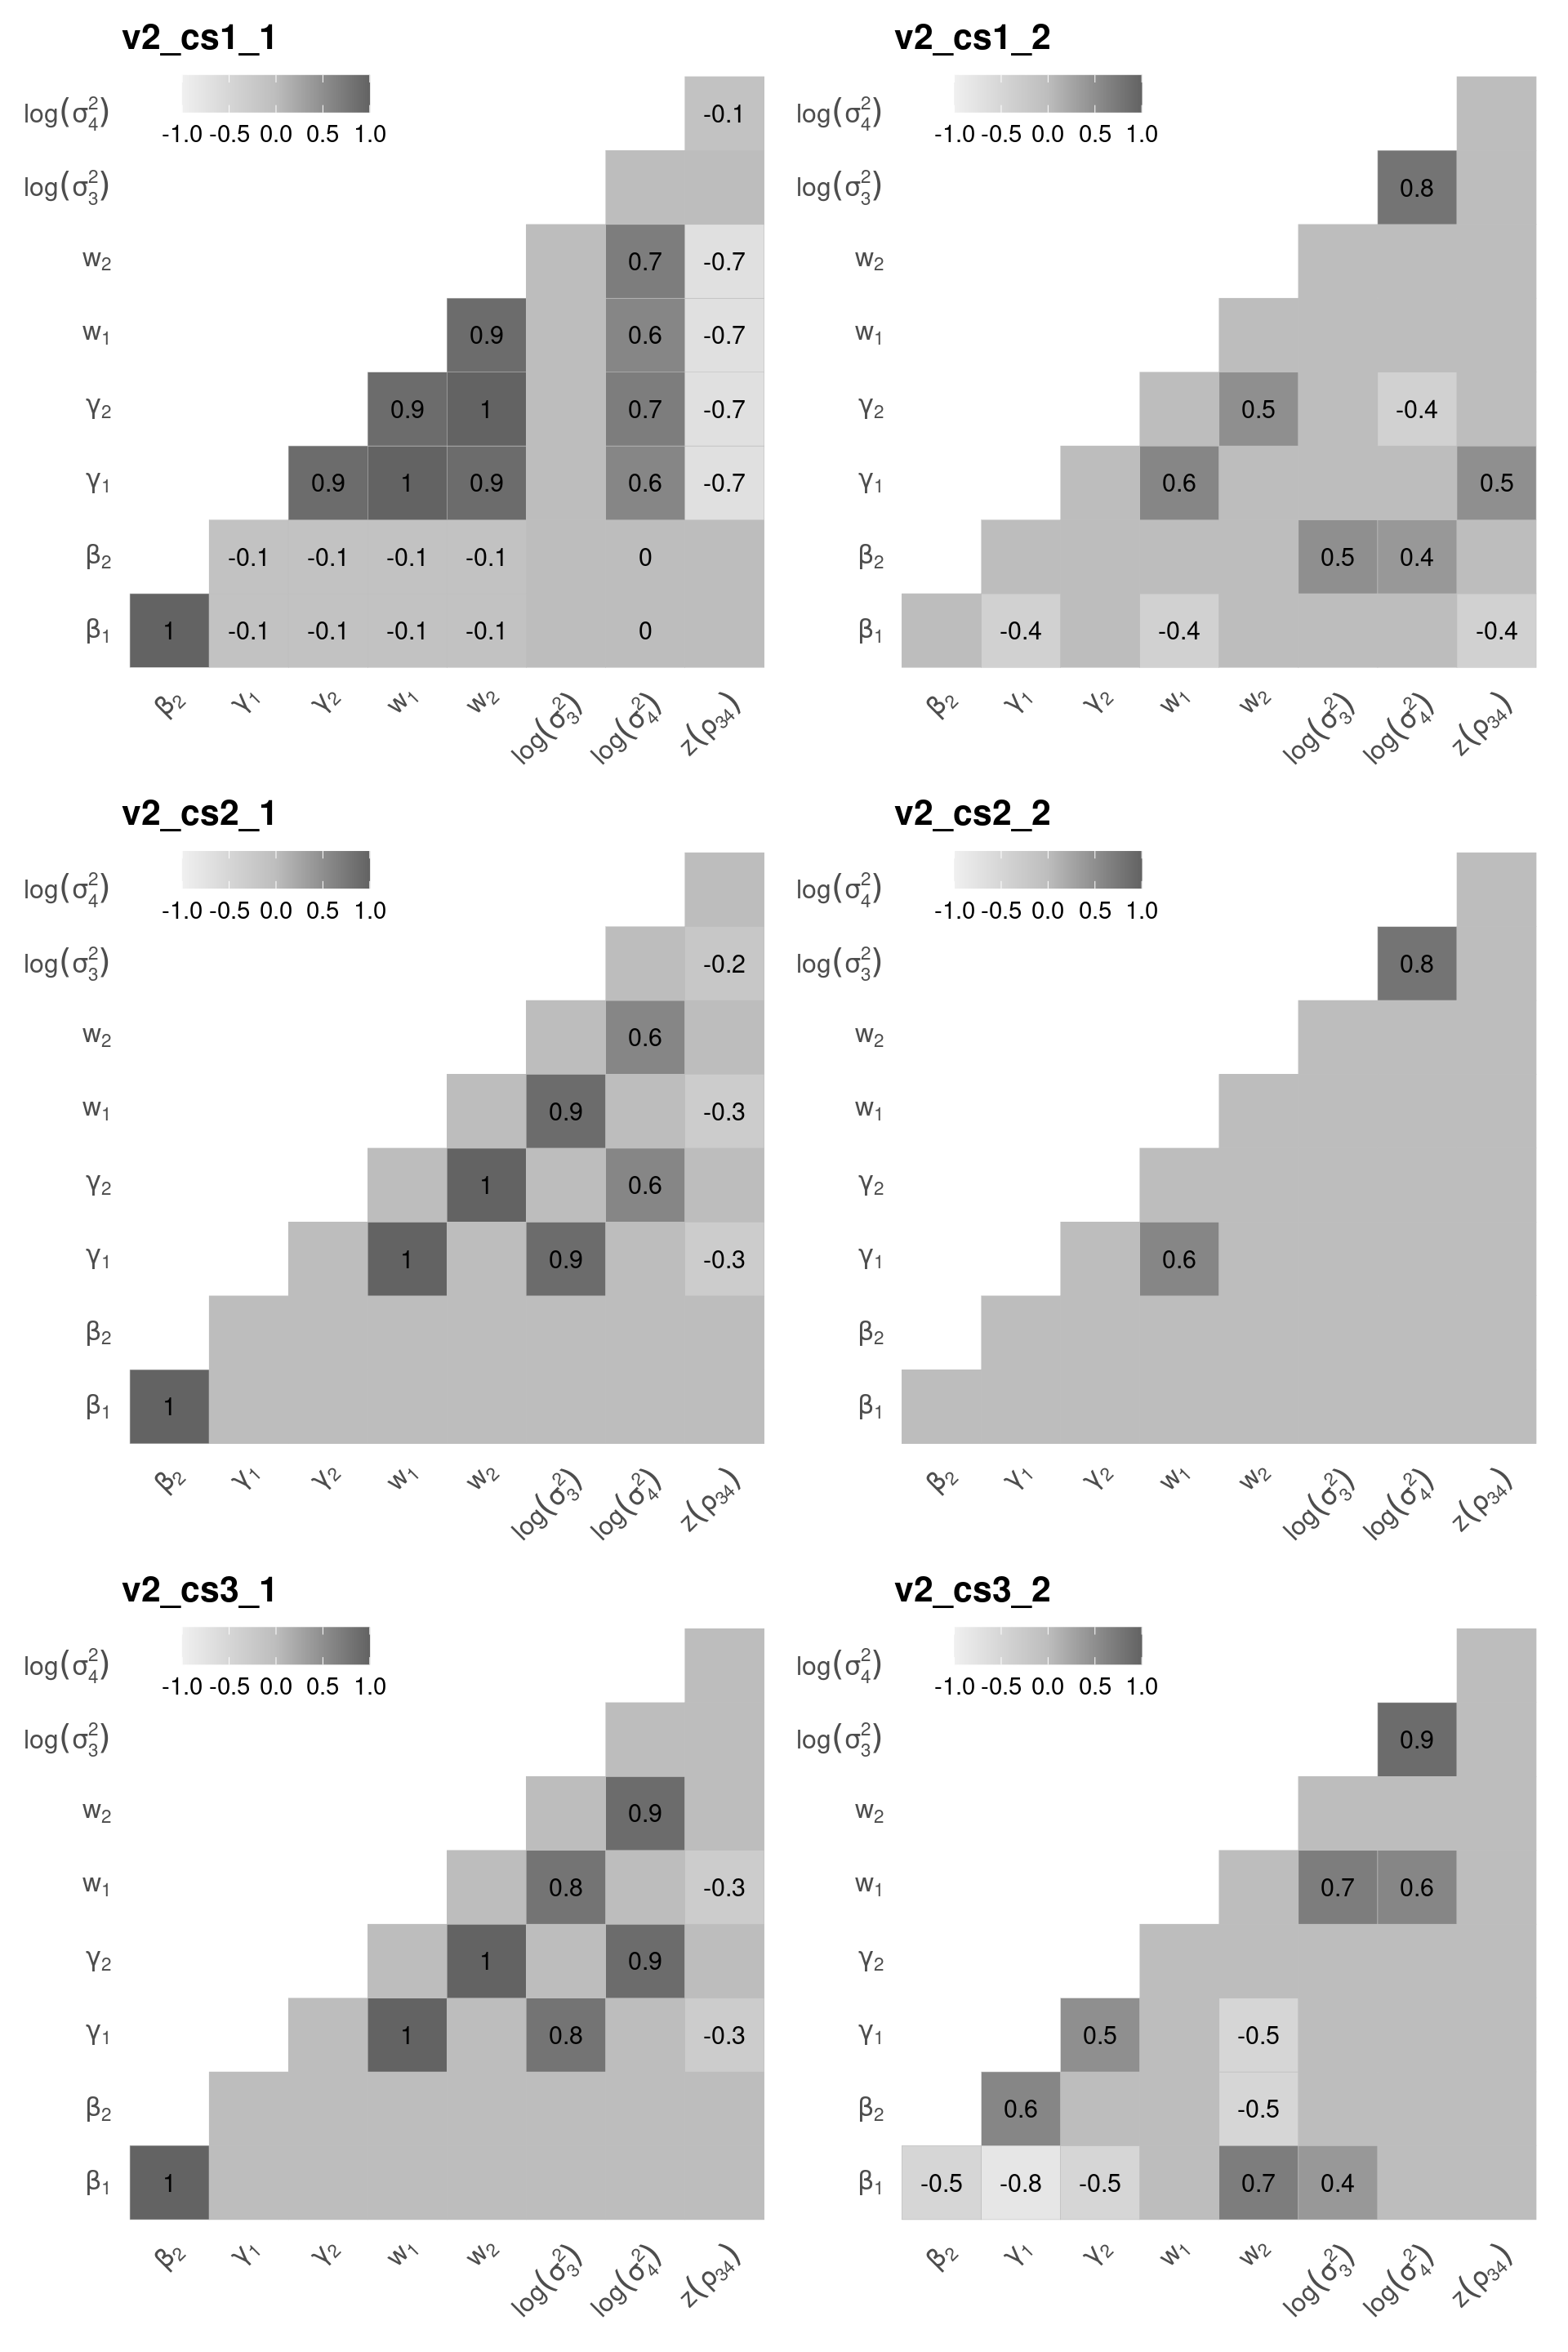
\includegraphics[width=\textwidth]{cor2plot-1.png}\\
 \begin{footnotesize}
  SOURCE: The author (2021).
 \end{footnotesize}
 \label{fig:cor2plot}
\end{figure}

\begin{figure}[H]
 \setlength{\abovecaptionskip}{.0001pt}
 \caption{VARIANCE-COVARIANCE MATRIX UPPER-TRIANGULAR COMPONENTS}
 \vspace{0.2cm}\centering
 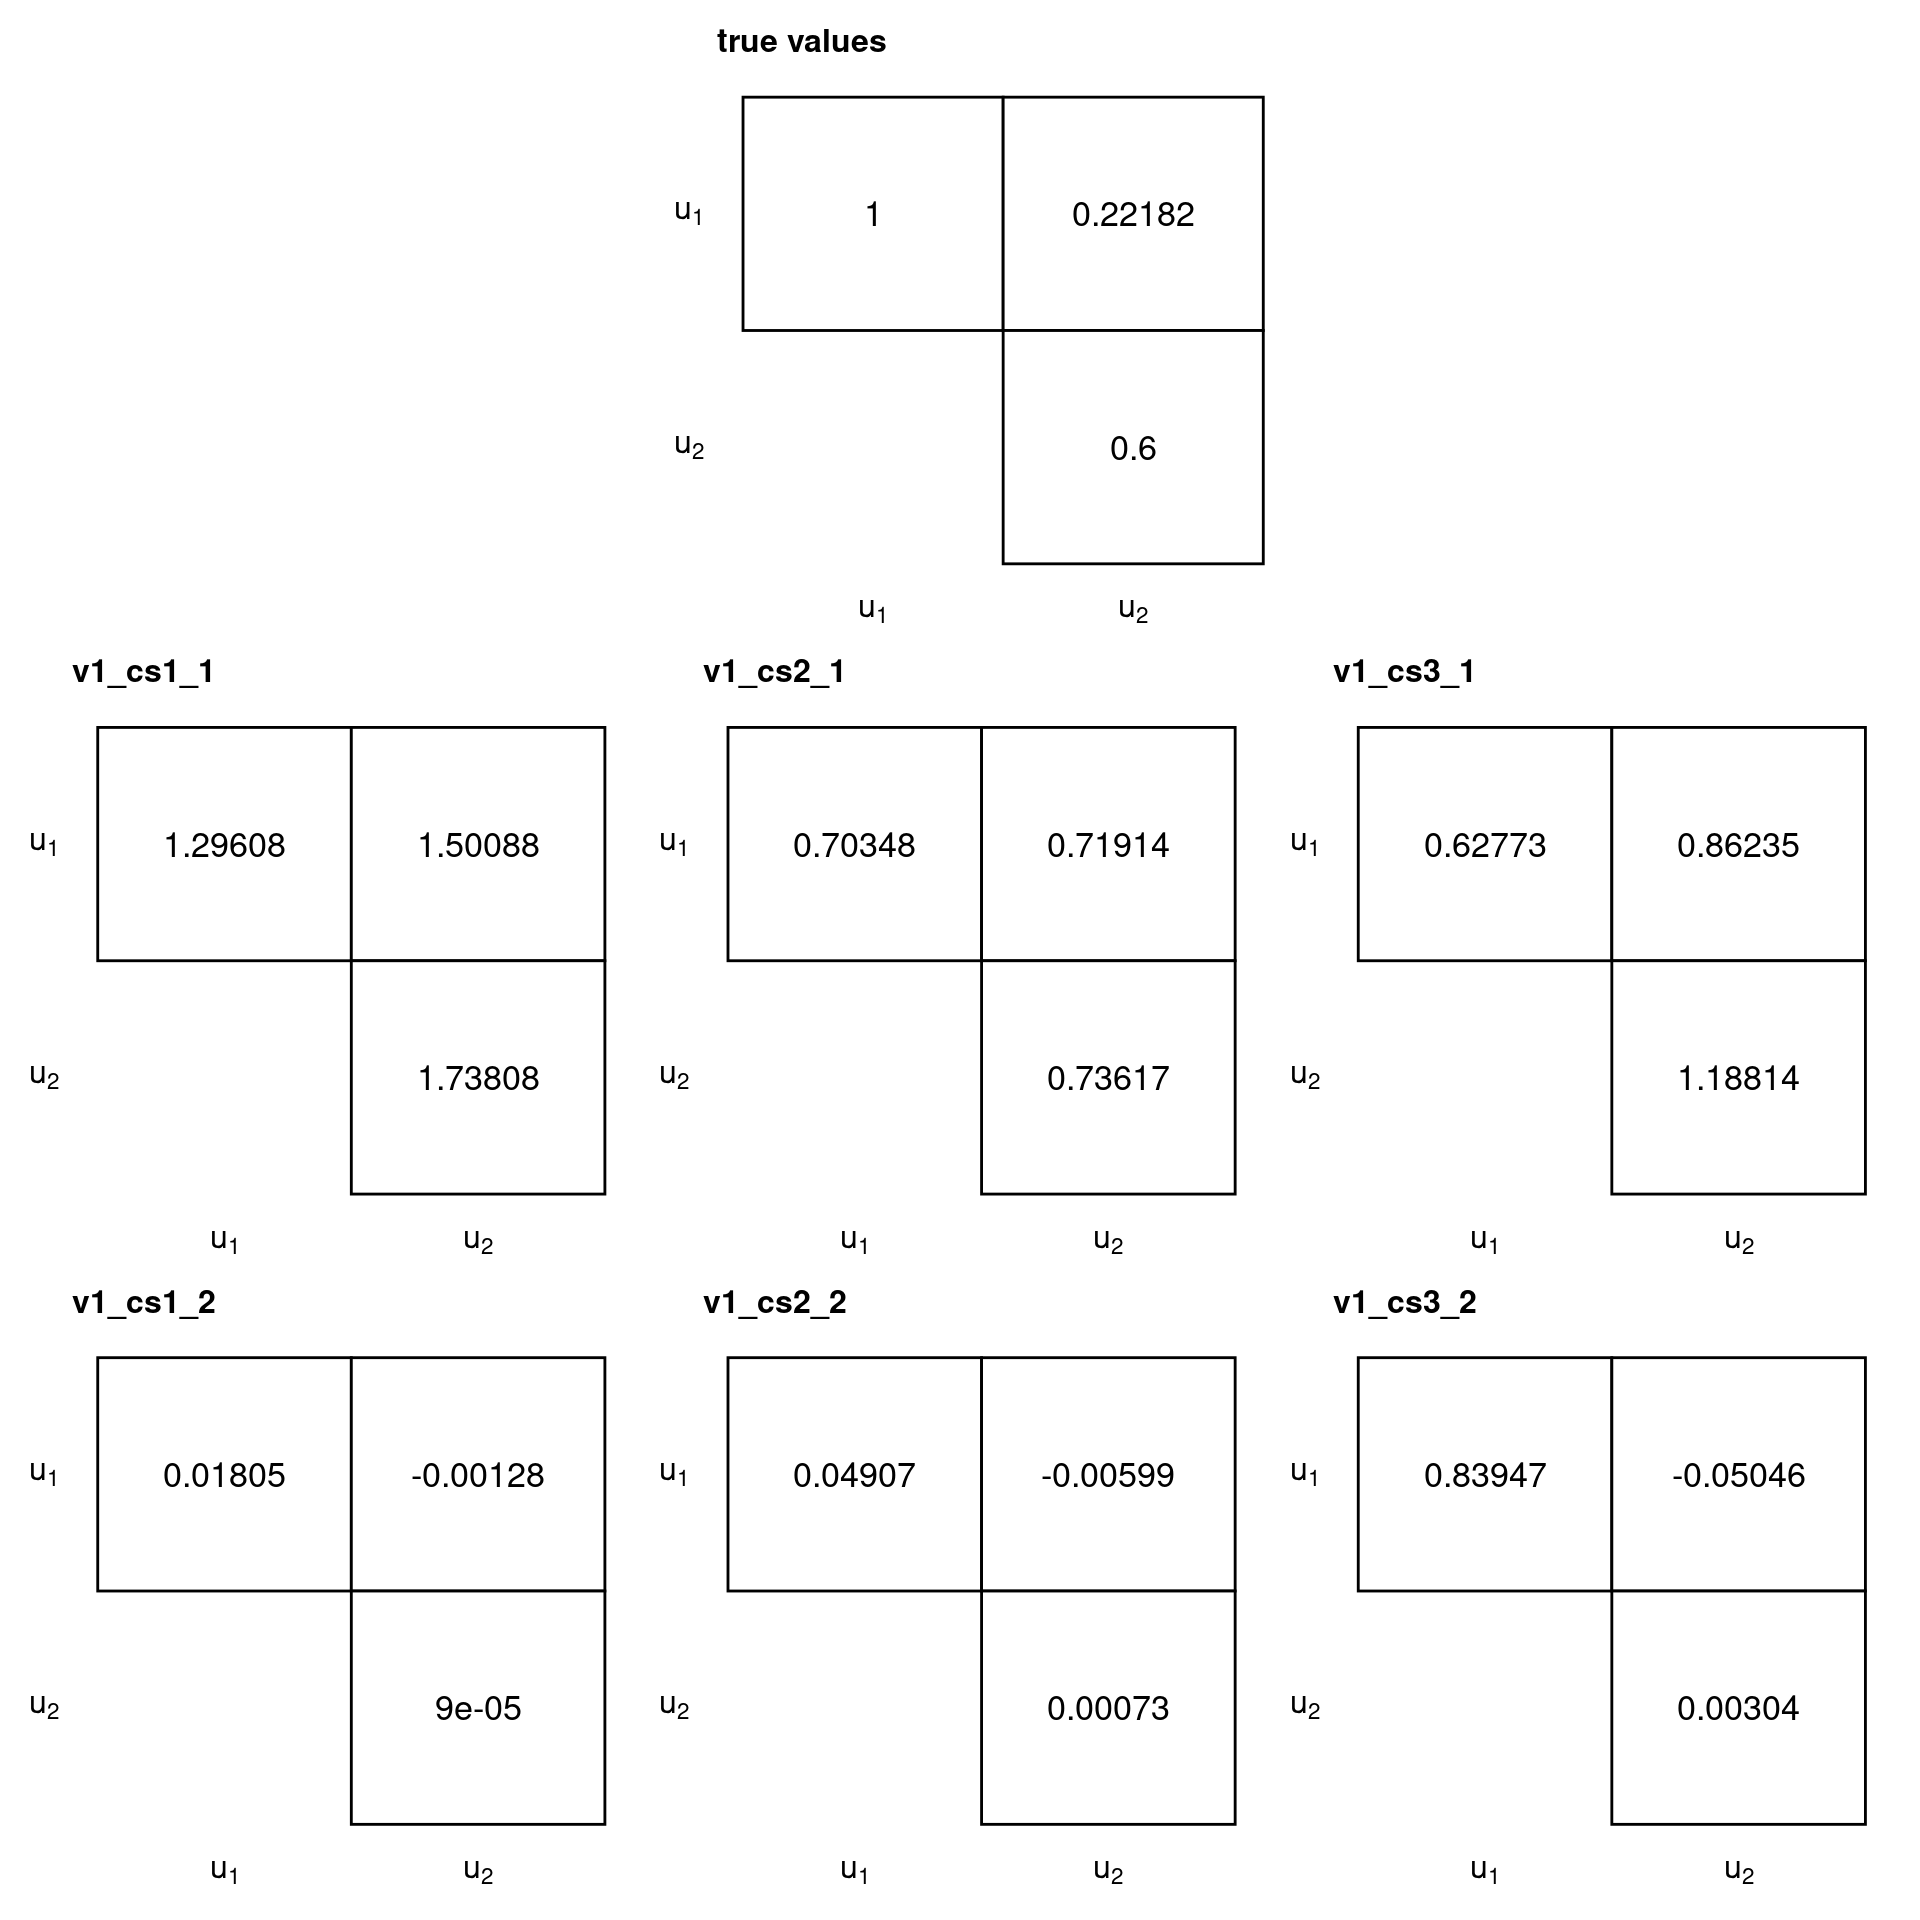
\includegraphics[width=\textwidth]{vcovs-1.png}\\
 \begin{footnotesize}
  SOURCE: The author (2021).
 \end{footnotesize}
 \label{fig:vcovs}
\end{figure}

\begin{figure}[H]
 \setlength{\abovecaptionskip}{.0001pt}
 \caption{CUMULATIVE INCIDENCE FUNCTIONS (CIFs)}
 \vspace{0.2cm}\centering
 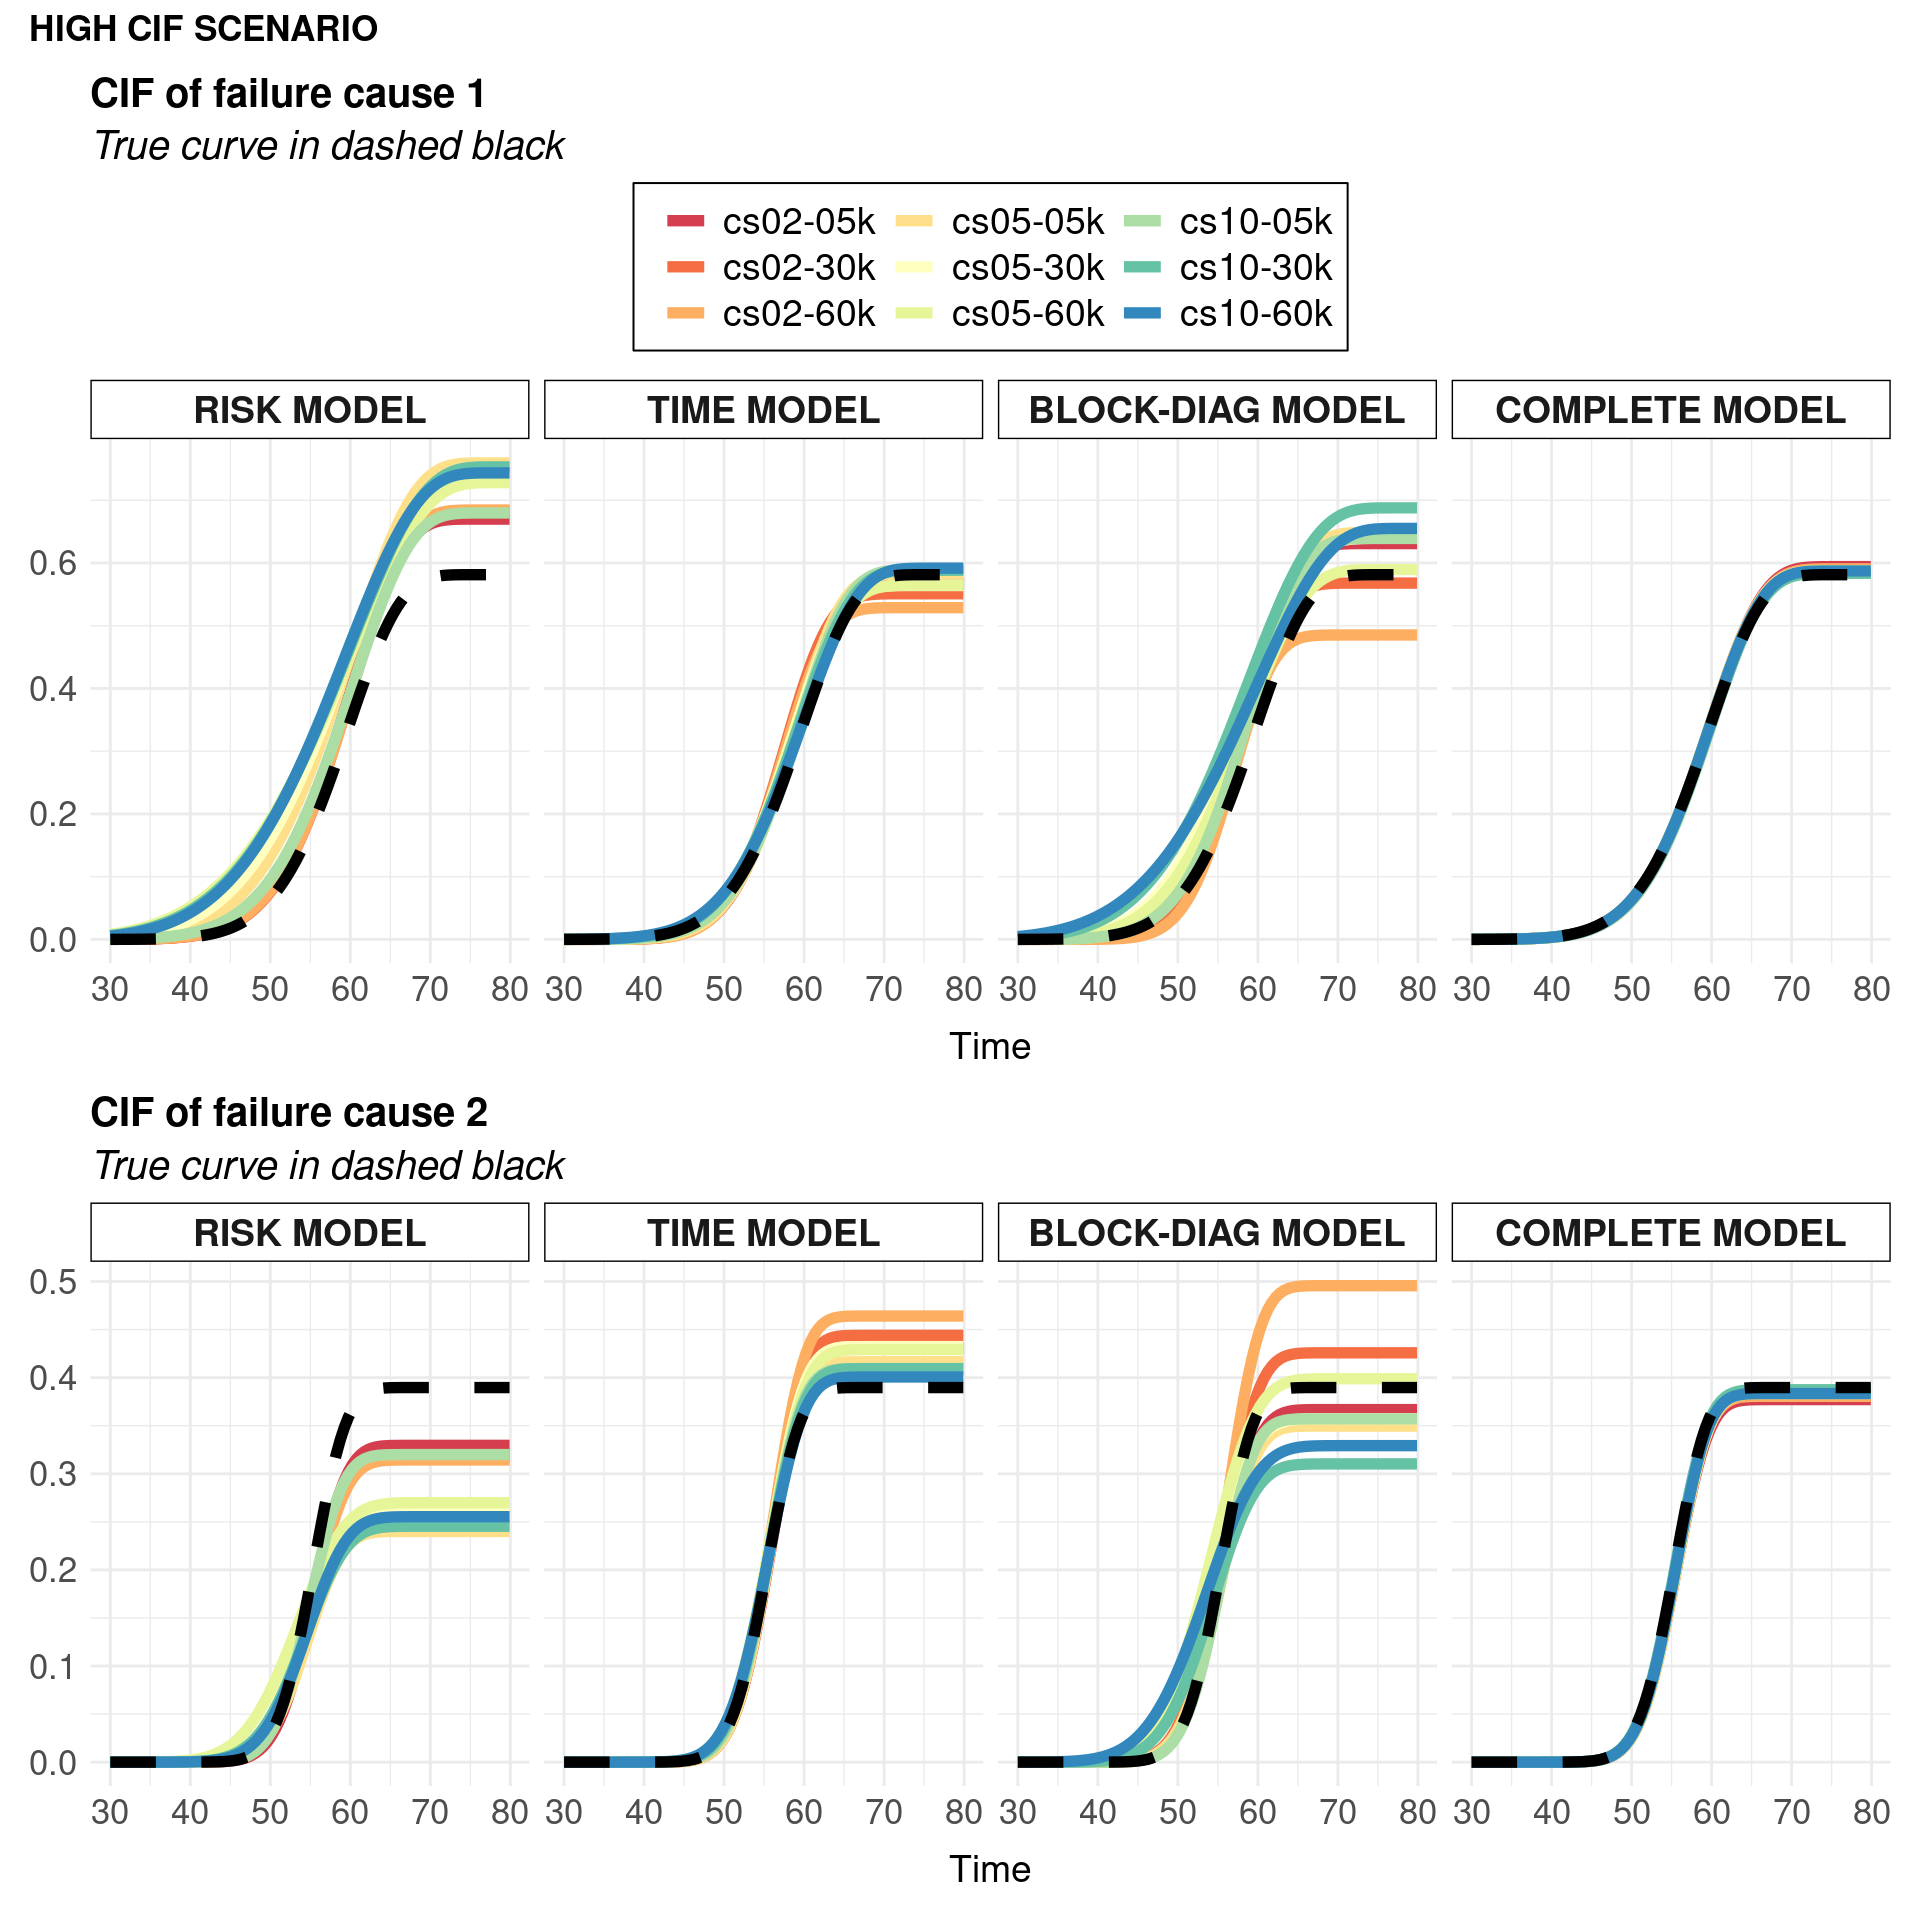
\includegraphics[width=\textwidth]{cifs-1.png}\\
 \begin{footnotesize}
  SOURCE: The author (2021).
 \end{footnotesize}
 \label{fig:cifs}
\end{figure}

\section{REAL-BASED DATASET}
\label{cap:datares}

% END ==================================================================
